\documentclass[12pt]{article}  
% Эта строка — комментарий, она не будет показана в выходном файле  
\usepackage[left=1cm,right=1cm,
top=2cm,bottom=2cm,bindingoffset=0cm]{geometry}
\usepackage{ucs} 
\usepackage[utf8x]{inputenc} % Включаем поддержку UTF8  
\usepackage[russian]{babel}  % Включаем пакет для поддержки русского языка  
\usepackage{amsmath}
\usepackage{listings}
\usepackage{color}
\usepackage{tikz}
\usepackage{pgfplots}
\usepackage{graphicx}
\usepackage{csvsimple}

\definecolor{mygreen}{rgb}{0,0.6,0}
\definecolor{mygray}{rgb}{0.5,0.5,0.5}
\definecolor{mymauve}{rgb}{0.58,0,0.82}
\title{Отчет по лабораторной работе 5 \\ 
	По предмету “Анализ алгоритмов” \\
	По теме “Умножение матриц”
}  
\date{2018}  
\author{Фирсова Дарья ИУ7-56}

\begin{document}  
	\maketitle  
	\newpage
	\section*{Введение}
	В лабораторной работе изучаются алгоритмы умножения матриц. Рассмотрены алгоритмы: стандартный и улучшенный алгоритм Винограда.  Вычисления для каждого алгоритма выполняются параллельно. \\
	\textbf{Цель лабораторной работы:} анализ, реализация и сравнительный анализ времени работы алгоритмов для различных размеров исходных матриц и количества потоков. \\
\newpage

\section{Аналитеская часть}
В данном разделе приведены алгоритмы умножения.
\subsection{Описание алгоритмов}

\subsubsection{Стандартный алгоритм умножения }

Имеем две матрицы A и B размерностями M x N и N x Q соответственно. \\Тогда результирующей матрицей будет матрица С размером M x Q, где $c_{ij}$ = $\sum_{r=1}^n a_{ir}\cdot b_{rj} ,   (i = 0,1,2...m, j = 0,1,2...q)$.
\\
\\
\subsubsection{Алгоритм Винограда}
Пусть $i$-я строка матрицы A - вектор  $\vec{U}$, а $j$-й столбец матрицы B - вектор $\vec{V}$. \\
Тогда $C_{ij}$ = \begin{tabular}{|c|c|c|c|}
	\hline
	$u_{1}$  $u_{2}$  $u_{3}$  $u_{4}$ \\
	\hline
\end{tabular} $\cdot$ 
\begin{tabular}{|c|}
	\hline
	$v_{1}$ \\
	$v_{2}$  \\
	$v_{3}$   \\
	$v_{4}$  \\
	\hline
\end{tabular}
= $u_{1}$$v_{1}$ + $u_{2}$$v_{2}$ + $u_{3}$$v_{3}$ + $u_{4}$$v_{4}$ = \\
($u_{1}$+$v_{2}$)($u_{2}$$v_{1}$) + ($u_{3}$+$v_{4}$)($u_{4}$+$v_{3}$) - $u_{1}$$u_{2}$ - $u_{3}$$u_{4}$ - $v_{1}$$v_{2}$ - $v_{3}$$v_{4}$. \\

"Хвост" для  $\vec{U}$ вычисляется заранее и используется повтороно при умножении на каждый столбец матрицы B. Аналогично для вектора $\vec{V}$

Если вектора $\vec{U}$ и $\vec{V}$ нечетной длины, то к приведенным выше вычислениям, добавляем 
$C_{ij}$ += $U_{N-1}\cdot V_{N-1}, \forall i,j$
\\
\newpage
\section{Конструкторская часть}
В данном разделе представлены схемы алгоритмов 

\begin{figure}[ht!]
	\centering
	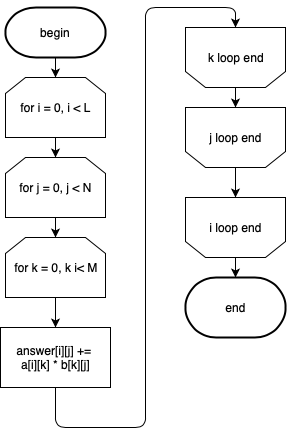
\includegraphics[width=70mm, height=120mm]{multiply.png}
	\caption{Схема стандартного алгоритма\label{overflow}}
\end{figure}
\newpage
\newpage
\begin{figure}[ht!]
	\centering
	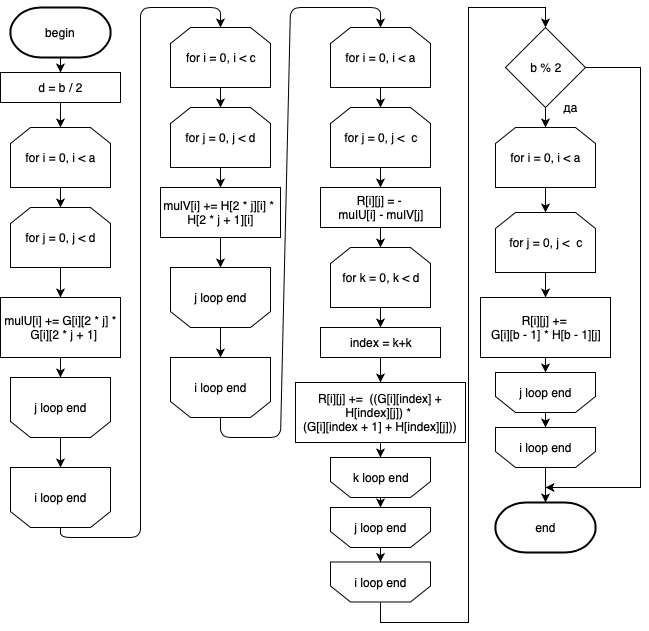
\includegraphics[width=150mm, height=150mm]{opt-2.png}
	\caption{Схема алгоритма улучшенного Винограда \label{overflow}}
\end{figure}

\newpage
\newpage

\section{Технологическая часть}

В этом разделе приведена реализация функций, указан язык программирования и необходимые модули. 
\subsection{Средства реализации}
В данной работе использовался язык Python 3.6, в среде Pycharm. Для измерения времени использовался модуль time, измерения производились в секундах.
Для параллельных вычислений использовался модуль threadind, метод Thread которого создает потоки с входными параметрами в виде имени функции и аргументов. 
\subsection{Листинг кода}
\lstset{ 
	backgroundcolor=\color{white},   % choose the background color; you must add \usepackage{color} or \usepackage{xcolor}; should come as last argument
	basicstyle=\footnotesize,        % the size of the fonts that are used for the code
	breakatwhitespace=false,         % sets if automatic breaks should only happen at whitespace
	breaklines=true,                 % sets automatic line breaking
	captionpos=b,                    % sets the caption-position to bottom
	commentstyle=\color{mygreen},    % comment style
	deletekeywords={...},            % if you want to delete keywords from the given language
	escapeinside={\%*}{*)},          % if you want to add LaTeX within your code
	extendedchars=true,              % lets you use non-ASCII characters; for 8-bits encodings only, does not work with UTF-8
	frame=single,	                   % adds a frame around the code
	keepspaces=true,                 % keeps spaces in text, useful for keeping indentation of code (possibly needs columns=flexible)
	keywordstyle=\color{blue},       % keyword style
	language=Python,                 % the language of the code
	morekeywords={*,...},            % if you want to add more keywords to the set
	numbers=left,                    % where to put the line-numbers; possible values are (none, left, right)
	numbersep=5pt,                   % how far the line-numbers are from the code
	numberstyle=\tiny\color{mygray}, % the style that is used for the line-numbers
	rulecolor=\color{black},         % if not set, the frame-color may be changed on line-breaks within not-black text (e.g. comments (green here))
	showspaces=false,                % show spaces everywhere adding particular underscores; it overrides 'showstringspaces'
	showstringspaces=false,          % underline spaces within strings only
	showtabs=false,                  % show tabs within strings adding particular underscores
	stepnumber=1,                    % the step between two line-numbers. If it's 1, each line will be numbered
	stringstyle=\color{mymauve},     % string literal style
	tabsize=1,	                   % sets default tabsize to 2 spaces
	title=Листинг 1. Реализация алгоритмов.                   % show the filename of files included with \lstinputlisting; also try caption instead of title
}
\lstinputlisting[language=Python]{main.py}
\newpage

\newpage
\newpage

\section{Экспериментальная часть}
В данном разделе будут приведены примеры работы алгоритмов и произведены замеры времени. Тестирование производилось на компьютере с процессором Intel Core i5 (I5-6267U) и оперативной памятью 8 Гб. 
\subsection{Примеры работы}
Пример результата работы умножения матриц. Так как в данной реализации генерируются случайные значения, то для проверки результата использовалась библиотека Numpy. При одинаковых входных данных алгоритмы выдают одинаковый результат, который сравнивается с результатом умножния с помощью функции numpy.matmul(). Для вычисления используются квадратные матрицы.
\newline

{\centering
$$\begin{bmatrix} 
12 & 14 & 20 \\
24 & 14 & 16 \\
\end{bmatrix}
+
\begin{bmatrix} 
11 &15\\
8 & 15 \\
14 & 15 \\
\end{bmatrix}
=
\begin{bmatrix} 
524 & 690 \\
600 & 810 \\
\end{bmatrix}$$
}

\subsection{Сравнительный анализ}
Сравнение алгоритмов стандартного умножения и улучшенного алгоритма Винограда в зависимости от количества потоков. На графиках приведены замеры времени работы для матрицы. Каждый экперимент проводился 30 раз, результат - среднее арифметическое замеров времени. 
\newpage
Таблица результатов для стандартного алгоритма умножения\\
\\
\begin{tabular}{l|l|l}%
	\bfseries Length & \bfseries Threads & \bfseries Time% specify table head
	\csvreader[head to column names]{mulresult.csv}{}% use head of csv as column names
	{\\\hline\csvcoli& \csvcolii & \csvcoliii}% specify your coloumns here
\end{tabular}
\newpage
Таблица результатов для алгоритма Винограда\\
\\
\begin{tabular}{l|l|l}%
	\bfseries Length & \bfseries Threads & \bfseries Time% specify table head
	\csvreader[head to column names]{winoresult.csv}{}% use head of csv as column names
	{\\\hline\csvcoli& \csvcolii & \csvcoliii}% specify your coloumns here
\end{tabular}
\newpage
\subsection{Вывод}
В результате эксперимента подтвердилось, что вычисления при нескольких потоках быстрее. Различие во времени выполнения связано с тем, что матрицы генерируются случайно.  Наиболее быстрыми оказались вычисления на 2 и 8 потоках. При увеличении значения потоков больше 10, производительность падает, поэтому контрольные замеры времени не производились. 

\newpage
\section{Заключение}
В лабораторной работе разработаны алгоритмы параллельного вычисления для умножения матриц.  Разработаны программы по этим алгоритмам, проведены тесты по времени, произведен сравнительный анализ алгоритмов. Для составления отчета использован Latex.
\\
\end{document}